% Copyright 2004 by Till Tantau <tantau@users.sourceforge.net>.
%
% In principle, this file can be redistributed and/or modified under
% the terms of the GNU Public License, version 2.
%
% However, this file is supposed to be a template to be modified
% for your own needs. For this reason, if you use this file as a
% template and not specifically distribute it as part of a another
% package/program, I grant the extra permission to freely copy and
% modify this file as you see fit and even to delete this copyright
% notice. 

\documentclass{beamer}

\usepackage{xcolor}
\usepackage{CJKutf8}
\usepackage{rotating}
\usepackage{subfigure}
\usepackage{graphicx}
\usepackage{algorithm}
\usepackage{algorithmicx}
\usepackage{amsmath}
\usepackage{amssymb}
\usepackage{algpseudocode}
\usepackage{wallpaper}
\algdef{SE}[DOWHILE]{Do}{DoWhile}{\algorithmicdo}[1]{\algorithmicwhile\ #1}%

\usetheme{Madrid} % origin
\setbeamercolor{structure}{fg=violet}

\author{Chi-Ming~Lee}

\institute[NTHU EE] % (optional, but mostly needed)
{
    Department of Electrial Engineering\\
    National Tsing Hua University
}

\date{\today}

\AtBeginSubsection[]
{
    \begin{frame}<beamer>{Outline}
        \tableofcontents[currentsection,currentsubsection]
    \end{frame}
}

\begin{document}
\setbeamertemplate{background canvas}{\CenterWallPaper{.30}{./assets/nthu_watermark.eps}}
\begin{CJK}{UTF8}{bkai}

    \title[DeAr DSP]{ DeAr: 適用於異質系統架構之高效率且彈性的數位訊號處理器設計}
    \subtitle{DeAr: An Efficient and Flexible Digital Signal Processor Design for Heterogeneous System Architecture}

    \begin{frame}
        \titlepage
    \end{frame}

    \begin{frame}{Outline}
        \tableofcontents
        % You might wish to add the option [pausesections]
    \end{frame}

    % Section and subsections will appear in the presentation overview
    % and table of contents.

    \section{Introduction}

    \subsection{Motivation}

    \begin{frame}{Motivation (1/2)}
        \begin{itemize}
            \item {
                    The evolution of wireless communication standard drives the quest on a new DSP architecture.
                }
            \item {
                    LTE-A demands 10 times transmission throughput than that of LTE. As a result...
                    \begin{itemize}
                        \item {
                                More sophisticated arithmetics are needed (throughput).
                            }
                        \item {
                                Algorithms for demodulation need to evolve rapidly (flexibility).
                        }
                        \item {
                                Endurance of embedded devices still matters (power-efficiency).
                        }
                    \end{itemize}
                }
            \item {
                    Conventional DSP architectures, VLIW and ASIP, are opposite extreme cases for processor design.
                }
        \end{itemize}
    \end{frame}

    \begin{frame}{Motivation (2/2)}
        \begin{itemize}
            \item {
                    Heterogeneous computing, a system with multiple types of processors, is gaining momentum.
                    \begin{itemize}
                        \item {
                                CPU handles control-intensive tasks.
                            }
                        \item {
                                DSP, GPU and FPGA handles data-intensive tasks.
                            }
                        \end{itemize}
                }
            \item {
                    Industry standard for heterogeneous computing, \textit{Heterogeneous System Architecture} emerged in 2012.
                    \begin{itemize}
                        \item {
                                Proposed by leading semiconductor companies, AMD, ARM, MediaTek, Samsung etc, 
                            }
                        \item {
                                It has opened a new era for embedded computing platforms.
                            }
                        \end{itemize}
                }
        \end{itemize}
    \end{frame}


    \subsection{Contribution}

    \begin{frame}{Contribution}
        \begin{itemize}
            \item {
                    We propose Dual-thread Architecture (DeAr) for DSP, which achieves both power-efficiency and flexibility.
                    \begin{itemize}
                        \item {
                                The multi-issue datapath manipulating Simultaneous Multi-threading (SMT).
                            }
                        \item {
                                Multi-banked register file (RF) with implicit RF addressing.
                            }
                        \item {
                                Transport-triggered data bus for exhaustive data forwarding.
                            }
                        \end{itemize}
                }
            \item {
                    We propose a framework to integrate DeAr DSP with an HSA platform.
                    \begin{itemize}
                        \item {
                                HSA compatible system integration framework.
                            }
                        \item {
                                HSA compatible compilation framework.
                            }
                        \end{itemize}
                }
            \item{
        Compared with VLIW and ASIP respectively, DeAr saves: 
                    \begin{itemize}
                        \item {
                            20.3\%--13.1\% and 31.8\%--2.2\% of power, 36.1\%--31.5\% and 28.2\%--5.7\% of area in the 1st benchmark suit.
                            }
                        \item {
                            20.3\%--13.1\% and 31.8\%--2.2\% of power, 36.1\%--31.5\% and 28.2\%--5.7\% of area in the 2nd benchmark suit.
                            }
                        \end{itemize}
                }
        \end{itemize}
    \end{frame}

    \section{Background}
    \subsection{Common DSP architectures}
    \begin{frame}{Very Long Instruction Word (VLIW)}
       \begin{columns}
           \begin{column}{0.5\textwidth}
               \begin{figure}[!ht]
                   \centering
                   \includegraphics[width=0.9\textwidth]{./figs/vliw.eps}
                   \caption{VLIW example}
               \end{figure}
           \end{column}
           \begin{column}{0.5\textwidth}
              \begin{itemize}
                  \item foo
                  \item bar
              \end{itemize} 
           \end{column}
       \end{columns} 
    \end{frame}

    \begin{frame}{Application Specific Instruction Set Processor (ASIP)}
        \begin{columns}
            \begin{column}{0.5\textwidth}
                \begin{figure}[!ht]
                    \centering
                    \includegraphics[width=0.9\linewidth]{./figs/cascade.eps}
                    \caption{ASIP example}
                \end{figure}
            \end{column}
            \begin{column}{0.5\textwidth}
               \begin{itemize}
                   \item foo
                   \item bar
               \end{itemize} 
            \end{column}
        \end{columns} 
    \end{frame}
    \begin{frame}{Transport-triggered Architecture (TTA)}
        \begin{itemize}
            \item foo
            \item bar
        \end{itemize}
        \begin{figure}[!ht]
            \centering
            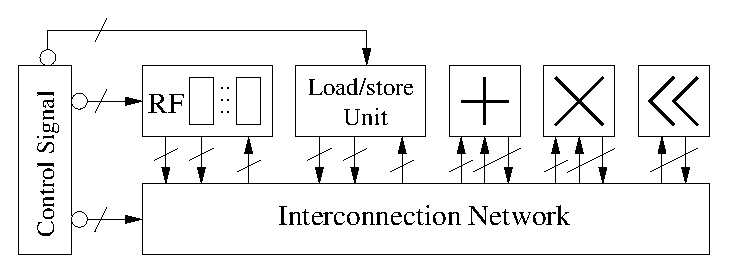
\includegraphics[width=0.6\linewidth]{./figs/tta.eps}
            \caption{TTA example}
        \end{figure}
    \end{frame}

    \subsection{Heterogeneous System Architecture}
    \begin{frame}{Key Concepts of HSA}
       \begin{itemize}
           \item Heterogeneous multi-core platform
           \item Heterogeneous System Architecture Intermediate Language (HSAIL)
           \item Shared Virtual Memory (SVM)
           \item Architectural Queuing Language (AQL)
       \end{itemize} 
    \end{frame}

    \begin{frame}{HSA platform example}
        \begin{figure}[!ht]
            \centering
            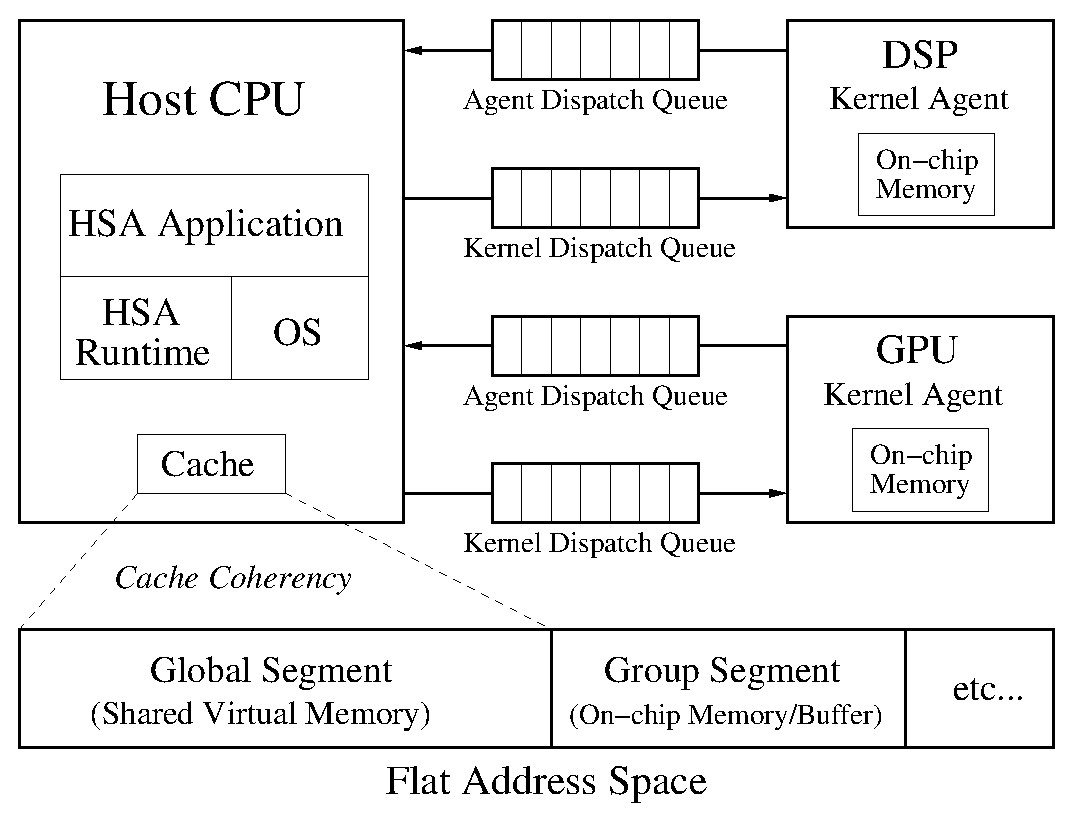
\includegraphics[width=0.8\textwidth]{./figs/systemspec.eps}
            \label{fig:systemspec}
        \end{figure}
    \end{frame}

    \begin{frame}{Execution hierarchy}
        \begin{figure}[!ht] 
            \centering
            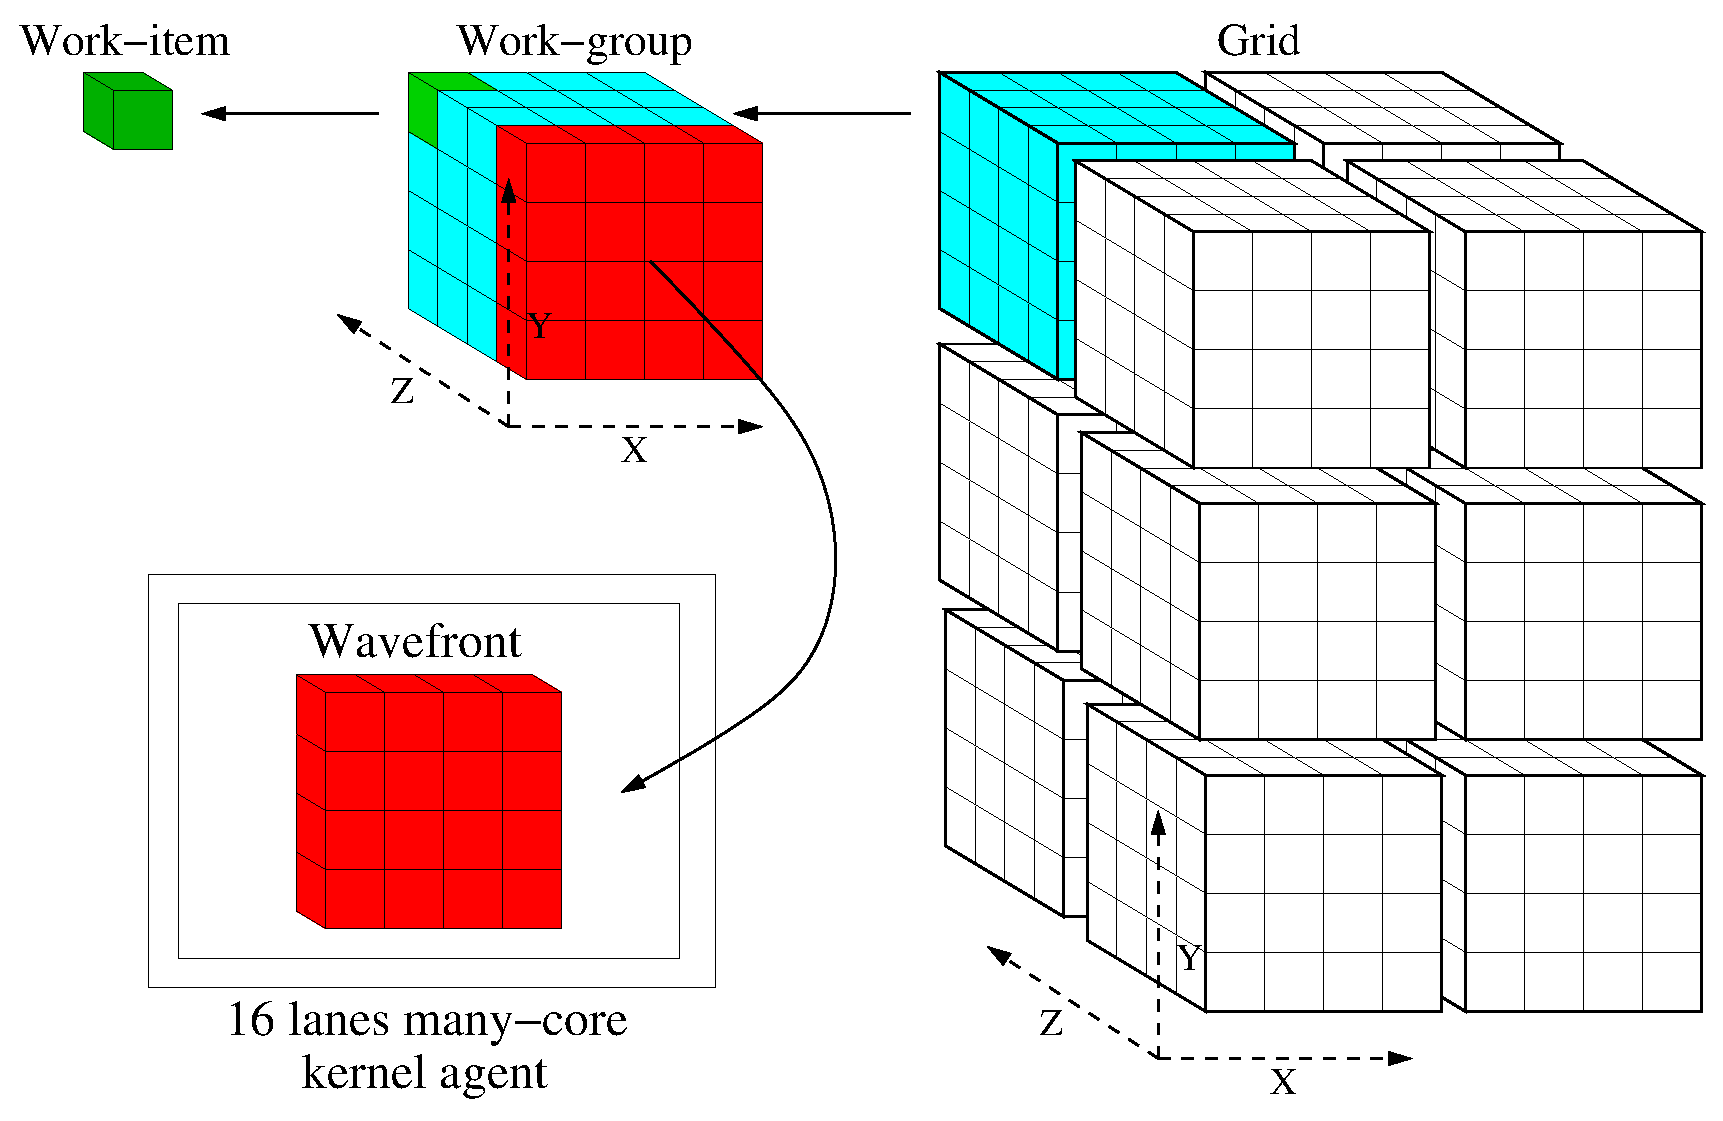
\includegraphics[width=0.8\textwidth]{./figs/grid.eps}
            \label{fig:grid}
        \end{figure}
    \end{frame}

    \begin{frame}{Software Infrastructure of HSA}
        \begin{figure}[!ht] 
            \centering
            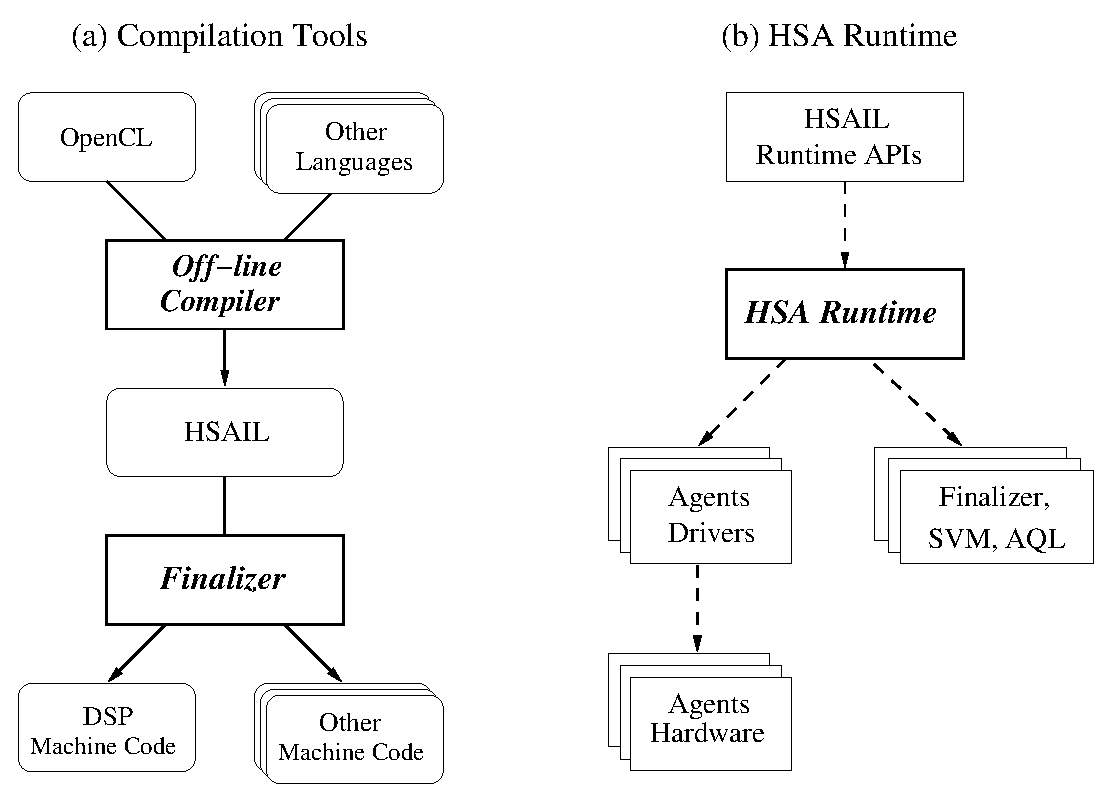
\includegraphics[width=0.8\textwidth]{./figs/swinf.eps}
            \label{fig:swinf}
        \end{figure}
    \end{frame}


    \section{Design and Implementation}
    \subsection{Proposed Architecture}

    \begin{frame}{System Integration (1/2)}
        \begin{figure}[!ht] 
            \centering
            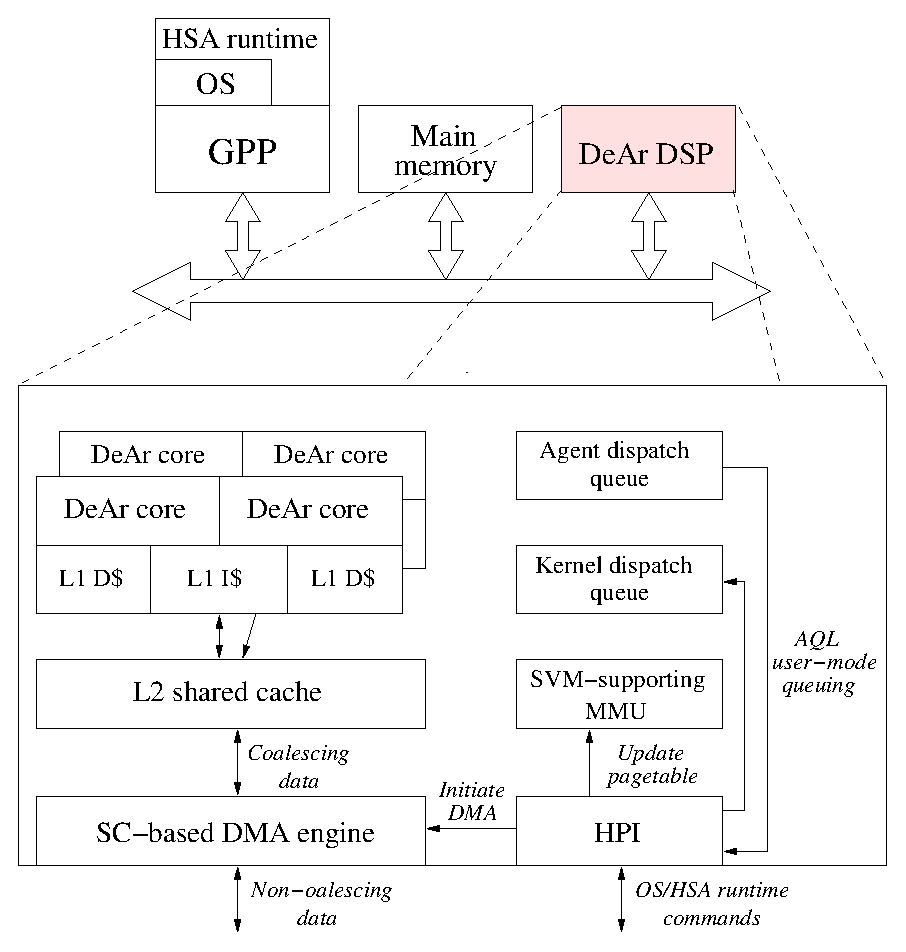
\includegraphics[width=0.5\textwidth]{./figs/archi.eps}
            \label{fig:archi}
        \end{figure}
    \end{frame}

    \begin{frame}{System Integration (2/2)}
        \begin{itemize}
            \item {
                    \textbf{MMU}: The host OS accesses MMU via HPI, and thus HSA SVM can be facilitated.
                }
            \item {
                    \textbf{Dispatch queues}: HSA runtime pushes (pops out) AQL-packets to (from) the kernel-dispatch queue (agent-dispatch queue) via HPI, 
                    and thus HSA user-mode queuing can be facilitated.
                }

            \item {
                    \textbf{SC}: The SC user API sends control signal to SC via HPI, 
                    and thus the data transfer and conversion fashion can be specified by the user.
                }
        \end{itemize}
    \end{frame}

    \begin{frame}{Concepts for Acceleration}
        \begin{figure}[!ht]
            \begin{center}
                \subfigure[Execution flow of an HSA work-item]
                {
                    \label{fig:bb:1}
                    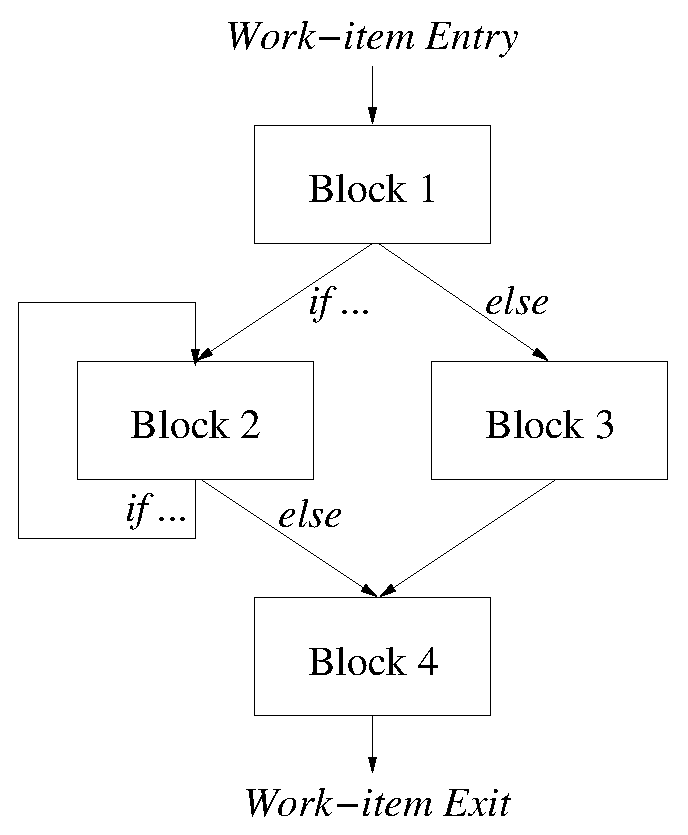
\includegraphics[width=0.3\textwidth]{figs/bb.eps}
                }
                \hfill
                \subfigure[Accelerating the execution of a Basic block]
                {
                    \label{fig:bb:2}
                    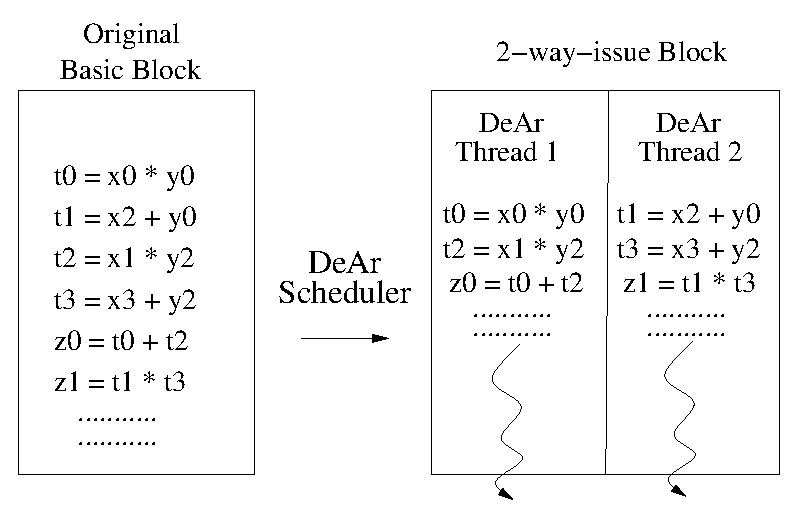
\includegraphics[width=0.55\textwidth]{figs/bb2.eps}
                }
            \end{center}
            \caption{Accelerating HSA with DeAr}
            \label{fig:bb}
        \end{figure}
    \end{frame}


    \subsection{Hardware Design and Implementation}
    \begin{frame}{Micro-architecture}
        \begin{figure}[!ht] 
            \centering
            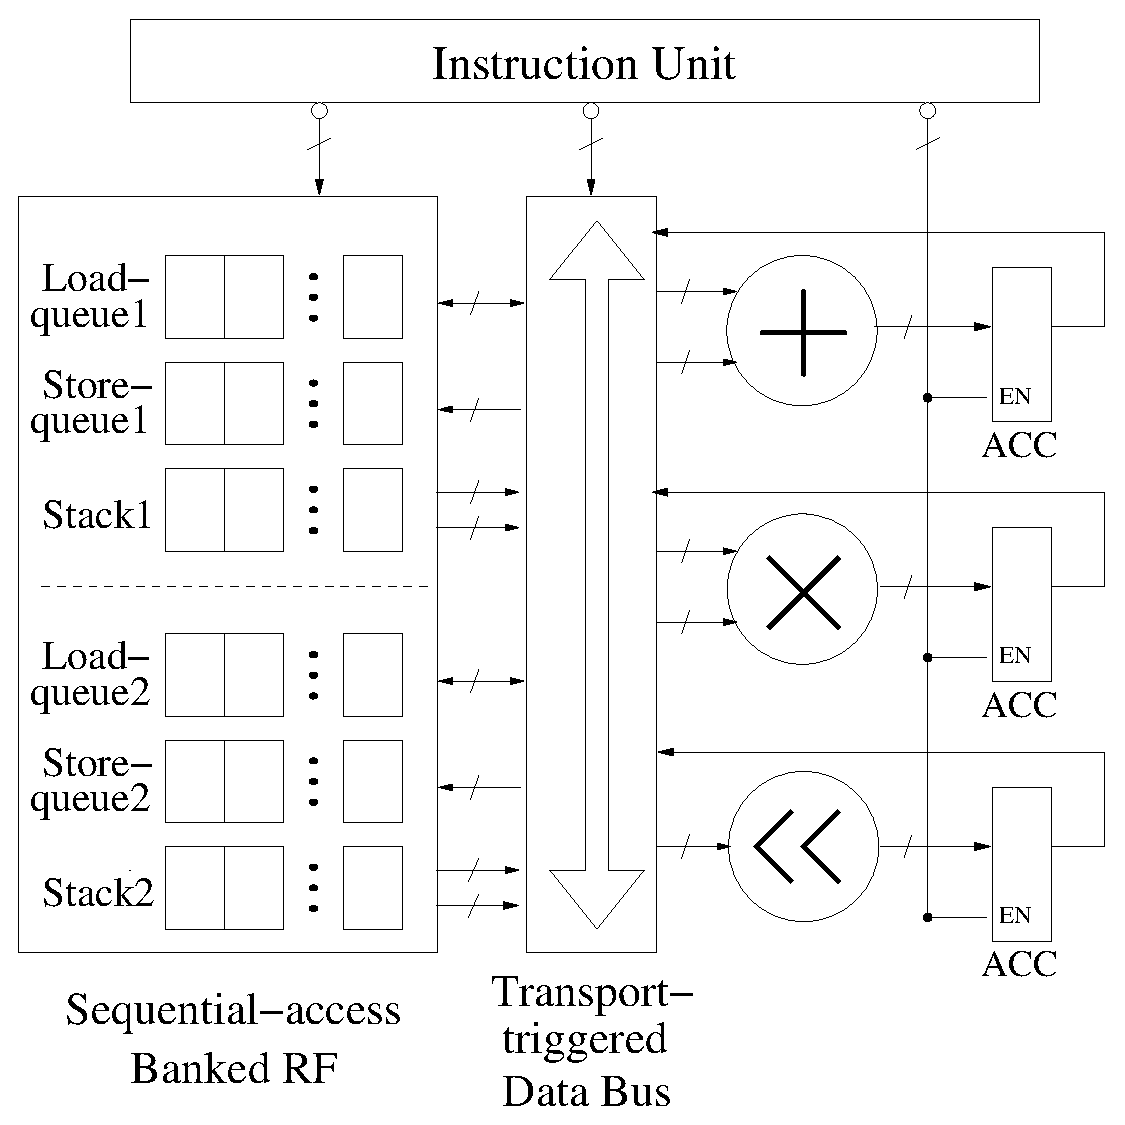
\includegraphics[width=0.6\textwidth]{./figs/micro.eps}
            \label{fig:micro}
        \end{figure}
    \end{frame}

    \begin{frame}{Instruction Set Architecture}
        
    \end{frame}
 
    \subsection{Software Design and Implementation}
    \begin{frame}{Data Flow Graph and Hierarchical Data Flow Graph}
        \begin{figure}[!ht]
            \begin{center}
                \subfigure[DFG example]
                {
                    \label{fig:dfg:dfg}
                    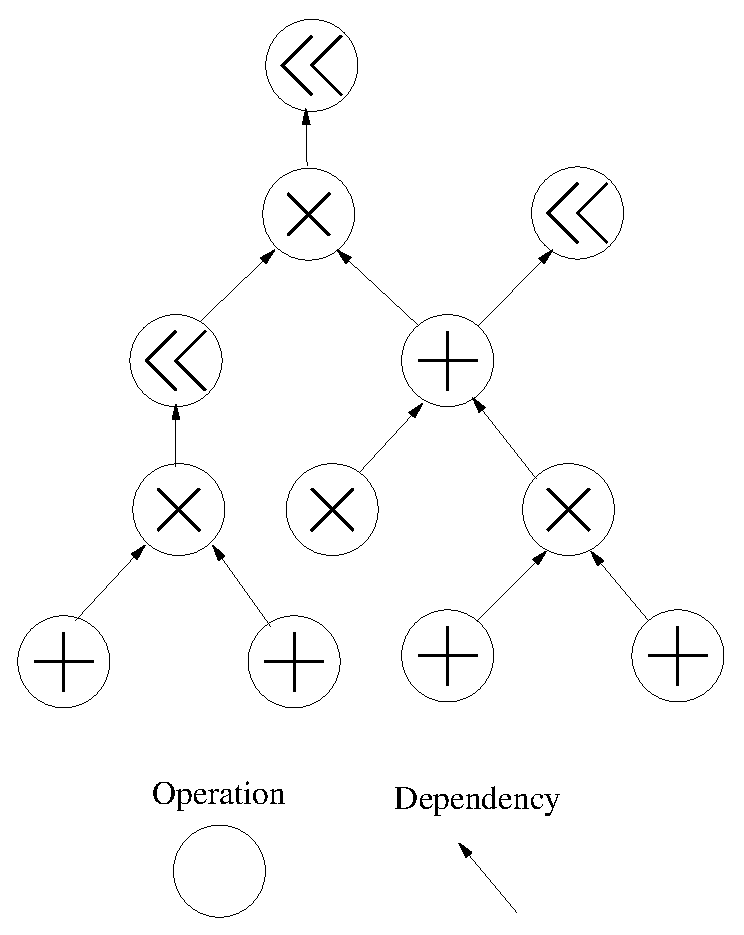
\includegraphics[width=0.4\textwidth]{figs/dfg.eps}
                }\hfill
                \subfigure[Corresponding HDFG]
                {
                    \label{fig:dfg:hdfg}
                    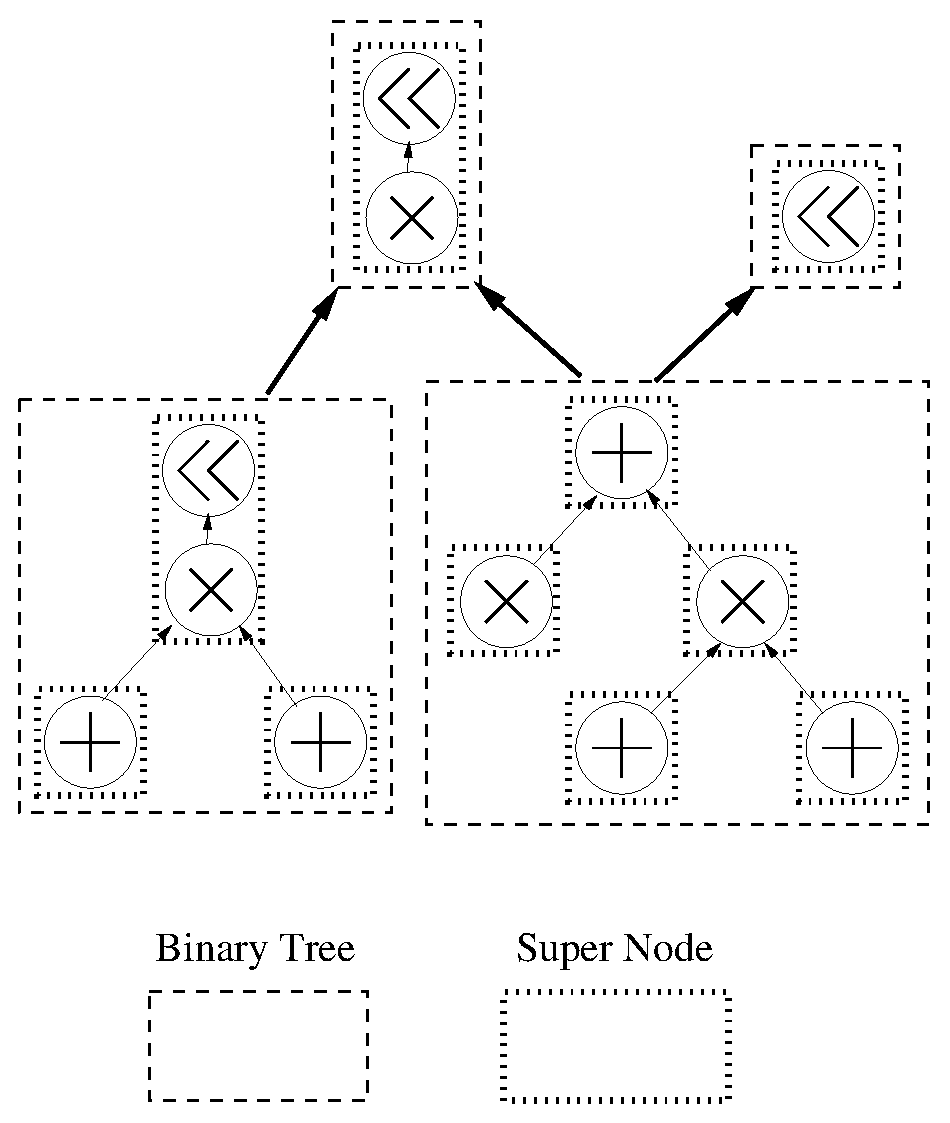
\includegraphics[width=0.4\textwidth]{figs/hdfg.eps}
                }
            \end{center}
            \label{fig:dfg}
        \end{figure}
    \end{frame}
    \begin{frame}{Properties of HDFG}
        
    \end{frame}
    \begin{frame}{HSAIL transformation (1/2)}
        
    \end{frame}

    \begin{frame}{HSAIL transformation (2/2)}
        
    \end{frame}

    \begin{frame}{HDFG-based scheduling (1/4)}
    \end{frame}
    
    \begin{frame}{HDFG-based scheduling (2/4)}
        
    \end{frame}

    \begin{frame}{HDFG-based scheduling (3/4)}
        \begin{figure}[!ht]
            \begin{center}
                \subfigure[Stage 1: scoring table modeling]
                {
                    \label{fig:alloc:1}
                    \includegraphics[width=0.3\textwidth]{figs/alloc.eps}
                }
                \hfill
                \subfigure[Stage 2: scoring table filling]
                {
                    \label{fig:alloc:2}
                    \includegraphics[width=0.3\textwidth]{figs/alloc2.eps}
                }
                \hfill
                \subfigure[Stage 3: backtracking]
                {
                    \label{fig:alloc:3}
                    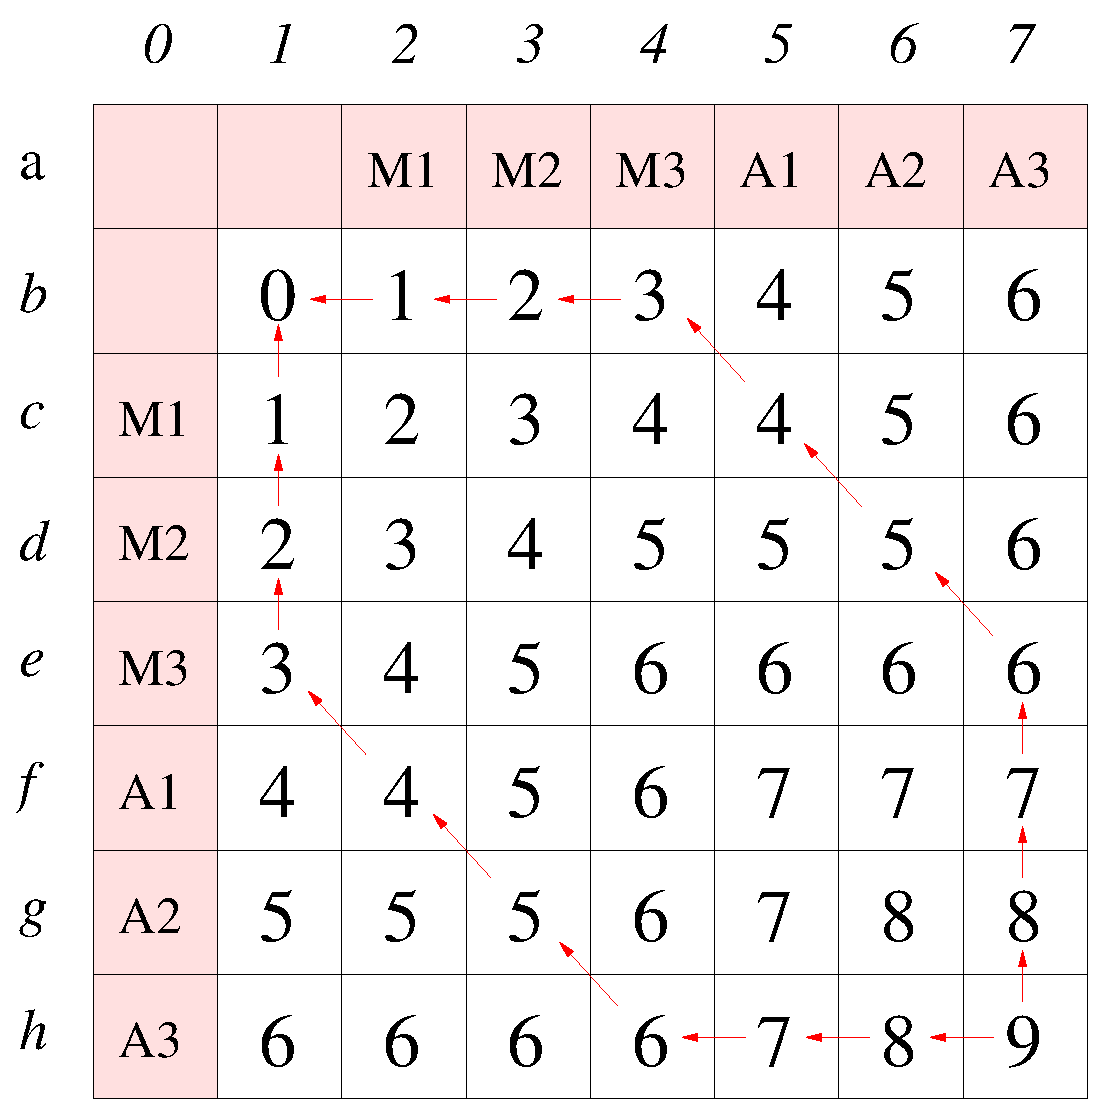
\includegraphics[width=0.3\textwidth]{figs/alloc3.eps}
                }
            \end{center}
            \label{fig:alloc}
        \end{figure}
    \end{frame}

    \begin{frame}{HDFG-based scheduling (4/4)}
        \begin{figure}[!h]
            \begin{center}
                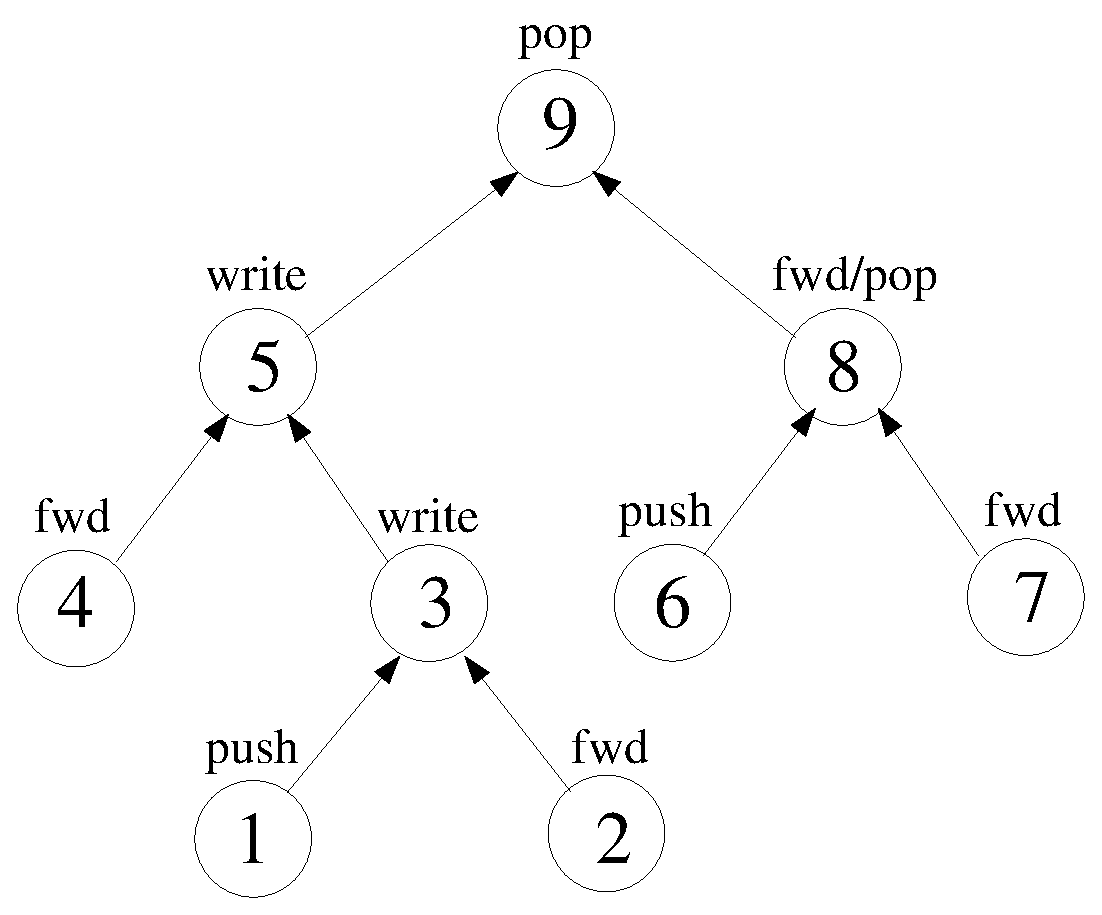
\includegraphics[width=0.6\textwidth]{figs/hfpt.eps}
            \end{center}
            \label{fig:hfpt}
        \end{figure}%
    \end{frame}
        
    \section{Performance Evaluation}
    \subsection{Experiment Setup}
    \begin{frame}{Why Single-core Evaluation?}
        
    \end{frame}
    \begin{frame}{Simulation Environment}
        
    \end{frame}

    \begin{frame}{Simulation Benchmark Suites}
        
    \end{frame}

    \subsection{Pre-synthesis Analysis}

    \begin{frame}{Operations per Cycle}
        
    \end{frame}

    \begin{frame}{Register File Access Rate}
        
    \end{frame}

    \subsection{Synthesis Result and Analysis}

    \begin{frame}{Area}
        
    \end{frame}

    \begin{frame}{Power Dissipation}
        
    \end{frame}

    \begin{frame}{Static Power Dissipation}
        
    \end{frame}

    \section{Conclusion and Future Work}
    \begin{frame}{Conclusion Remarks (1/2)}
        
    \end{frame}
    \begin{frame}{Conclusion Remarks (2/2)}
        
    \end{frame}
    \begin{frame}{Future Work (1/2)}
        
    \end{frame}

    \begin{frame}{Future Work (2/2)}
        
    \end{frame}
\end{CJK}
\end{document}


